\section{Relational cross-attention and the abstractor module}\label{sec:abstractor_module}

At a high level, the primary function of an Abstractor is to compute abstract relational features of its inputs.\footnote{In this paper, we will tend to use the name `Abstractor' to refer to both the module, the framework, and models which contain the Abstractor module as a main component.} That is, given a set or sequence of input objects $x_1, \ldots, x_\m$, the relational abstractor learns to model a relation $r(\cdot, \cdot)$ and computes a function on the set of pairwise relations between objects ${\{ r(x_i, x_j) \}}_{ij}$. At the heart of the abstractor module is an inductive bias we call the \textit{relational bottleneck}---it separates relational information from the features of individual objects.

%The relations modeled by the Abstractor and the computations on them are learned to carry out a specific prediction task. This learning is often end-to-end, but, crucially, the Abstractor framework naturally supports modular learning.

\subsection{Modeling relations as inner products}\label{ssec:relations_as_inner_prods}

A relation function is a function which maps a pair of objects $x_1, x_2 \in \calX$ to a vector representing the relation between the two objects. We model pairwise relations as inner products between appropriately encoded (or `filtered') object representations. In particular, we model the pairwise relation function $r(\cdot, \cdot) \in \mathbb{R}^{d_r}$ in terms $d_r$ learnable `left encoders' $\phi_1, \ldots, \phi_{d_r}$, and $d_r$ `right encoders' $\psi_1, \ldots, \psi_{d_r}$,
\begin{equation}\label{eq:inner_prod_rel}
    r(x_1,x_2) = \left(\langle \phi_1(x_1), \psi_1(x_2) \rangle, \langle \phi_2(x_1), \psi_2(x_2) \rangle, \ldots, \langle \phi_{d_r}(x_1), \psi_{d_r}(x_2) \rangle \right)^\top \in \mathbb{R}^{d_r}.
\end{equation}
A common choice is to model $(\phi_i, \psi_i)_{i\in [d_r]}$ as linear or affine maps, perhaps with a common non-linear encoder as a first step. Considering all pairwise relations yields a \textit{relation tensor}, $R = \left[r(x_i, x_j)\right]_{i,j} \in \mathbb{R}^{\m \times \m \times d_r}$.


In principle, relations could be modeled by an arbitrary learnable function applied to the concatenation of the features of a pair of objects.~\citep{santoro1} takes this approach and model relations through MLPs applied to the concatenation of the features of a pair of objects. This approach is versatile and can work given enough data. However, modeling relations as inner products has some important advantages. First, it enforces a relational bottleneck. When relations are modeled as $g_\theta(\mathrm{concat}(x_1, x_2))$, for some parameterized function class $g_\theta$, there is no pressure or restriction that this function represents relations between the two objects---it can just as well represent information about the objects' features individually. Modeling relations as inner products $\iprod{\phi(x_1)}{\psi(x_2)}$ ensures that the output represents a comparison between the two objects' features. Moreover precisely, inner product relations induce a geometry on the object space $\calX$. To see this, consider the case of symmetric relations. Then, the inner product $\iprod{\phi(x_1)}{\phi(x_2)}$ turns $\calX$ into an inner product space with well-defined notions of distance, angles, and orthogonality. Finally, modeling relations as inner products does not result in a loss of expressive power since inner product relations capture arbitrary continuous functions on $\calX \times \calX$ (see~\Cref{sec:function_classes}). Modeling relations as inner products is an approach that has been explored in previous work on relational architectures (e.g.,~\citep{esbn,kerg2022neural}) and has been shown to be a useful inductive bias on various relational tasks.

\subsection{Relational Cross-Attention}\label{ssec:relational_crossattention}

The core operation in a transformer is attention. For an input sequence $X = \paren{x_1, \ldots, x_\m}$, self-attention transforms the sequence via,

\begin{equation}\label{eq:self_attn}
    X' \gets \phi_v(X) \, \mathrm{Softmax}\paren{\phi_q(X)^\top \phi_k(X)},
\end{equation}

\noindent where $\phi_q, \phi_k, \phi_v$ are functions on $\calX$ applied elementwise to each object in the sequence (i.e., $\phi(X) = \paren{\phi(x_1), \ldots, \phi(x_\m)}$). Typically, those are linear or affine functions, with $\phi_q, \phi_k$ having the same dimensionality so we can take their inner product. Note that $\phi_q(X)^\top \phi_k(X)$ is a relation matrix in the sense defined above. Self-attention admits an interpretation as a form of message-passing. In particular, let $R = \mathrm{Softmax}\paren{\phi_q(X)^\top \phi_k(X)}$ be the softmax-normalized relation matrix. Then self-attention takes the form,

\begin{equation}\label{eq:self_attn_message_passing}
    \begin{split}
        x_i' &\gets \mathrm{MessagePassing}\paren{\set{(\phi_v(x_j), R_{ij})}_{j \in [\m]}}\\
        &= \sum_{j} R_{ij} \phi_v(x_j).
    \end{split}
\end{equation}

Thus, self-attention is a form of message-passing where the message from object $j$ to object $i$ is an encoding of object $j$'s features weighted by the (softmax-normalized) relation between the two objects. As a result, the processed representation obtained by self-attention involves some relational information. However, this relational information is entangled with the features of individual objects.

Our goal is to learn relational representations which are abstracted away from the features of individual objects in order to achieve more sample-efficient learning and improved generalization in relational reasoning. This is not naturally supported by entangled representations learned in standard self-attention. A key property of the Abstractor that enables enhanced relational processing is that it implements an inductive bias we call the \textit{relational bottleneck}. This is a type of information bottleneck which enforces that the Abstractor computes a purely relational representations, separating relational information from the features of individual objects.

We achieve this via a simple modification of attention---we replace the values $\phi_v(x_i)$ with input-independent vectors which identify the objects but do not encode any information about their features. We call those vectors \textit{symbols}. Hence, we make it so that the message from object $j$ to object $i$ is the symbol identifying object $j$, $s_j$, together with the relation between the two objects, $R_{ij}$.

\begin{equation}\label{eq:relational_crossattn_message_passing}
    \begin{split}
        A_i &\gets \mathrm{MessagePassing}\paren{\set{(s_j, R_{ij})}_{j \in [\m]}}\\
        &= \sum_{j} R_{ij} s_j.
    \end{split}
\end{equation}

Symbols act as abstract references to objects. They do not contain any information about the contents or features of the objects, but rather identify objects via their \textit{position}. The symbols $S = (s_1, s_2, \ldots)$ can be either learned parameters of the model or nonparametric positional embeddings (e.g., sinusoidal positional embeddings). Those vectors are `symbols' in the same sense that $x$is a symbol in an equation like $y = x^2$---they are a reference to an unspecified value. The difference is that the symbols in relational cross-attention are distributed representations (i.e., vectors), so this gives a novel perspective on the long-standing problem of neural versus symbol computation.

This modification yields a variant of attention which we call \textit{relational cross-attention},

\begin{equation}\label{eq:relational_crossattn}
    X' \gets S_{1:m} \, \sigma_{\mathrm{rel}}\paren{\phi(X)^\top \psi(X)},
\end{equation}

where $S$ are the input-independent symbols, $\sigma_{\mathrm{rel}}$ is the relation activation function, and $\phi, \psi$ correspond to the query and key transformations. When the relation activation function $\sigma_{\mathrm{rel}}$ is softmax, this corresponds to $\mathrm{Attention}(Q \gets X,\, K \gets X,\, V \gets S)$. By contrast, self-attention corresponds to $\mathrm{Attention}(Q \gets X,\, K \gets X,\, V \gets X)$, mixing sensory-information with representations of individual objects.

We observe in our experiments that allowing $\sigma_{\mathrm{rel}}$ to be a configurable hyperparameter can lead to performance benefits in some tasks. Softmax has the effect of normalizing the relation between a pair of objects $(i,j)$ based on the strength of $i$'s relations with the other objects in the sequence. In some tasks this is useful. In other tasks, this may mask relevant information. In that case, a tanh or sigmoid activation function may be more appropriate.

Relational cross-attention implements a type of information bottleneck, which we term the relational bottleneck, wherein relational cross-attention only represents relational information about the object sequence and does not encode information about individual objects. This enables a branch of the model to focus purely on modeling the relations between objects, yielding greater sample-efficiency in tasks which rely on relational reasoning.

\begin{remark}
    We call this operation ``relational cross-attention'' because 1) it computes relational representations, and 2) when attending to the input objects, it ``crosses'' a semi-permeable membrane which allows relational information to pass through but not sensory information about individual objects.
\end{remark}

In our experiments, $\phi_i, \psi_i$ are linear maps $W_1^{(i)}, W_2^{(i)}$. Relational cross-attention is given by,
\begin{equation}
    \begin{split}
        \mathrm{RelationalCrossAttention}(X, S) &= \mathrm{MultiHeadAttention}\paren{Q \gets X,\, K \gets X,\, V \gets S} \\
        &= W_o \, \mathrm{concat}\paren{A^{(1)}, \ldots, A^{(d_r)}}, \\
        \text{where } A^{(i)} &= W_o^{(i)} S \, \sigma_{\mathrm{rel}}\paren{(W_1^{(i)} X)^\top (W_2^{(i)} X)}.
    \end{split}
\end{equation}

% TODO: FIGURE COMPARING DIFFERENT ATTENTION MECHANISMS
\begin{figure}
    \begin{subfigure}[b]{0.5\textwidth}
        \centering
        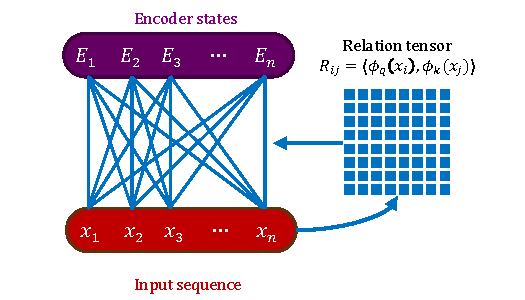
\includegraphics[width=\textwidth]{figures/self_attn_fig.pdf}
        \caption{$E \gets \mathrm{SelfAttention}(X)$}
        \label{fig:self_attention}
    \end{subfigure}
    \hfill
    \begin{subfigure}[b]{0.5\textwidth}
        \centering
        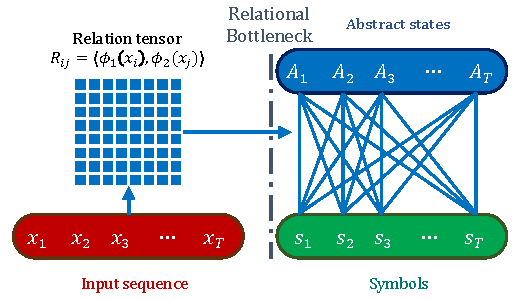
\includegraphics[width=\textwidth]{figures/rel_crossattn_fig.pdf}
        \caption{$A \gets \mathrm{RelationalCrossAttention(X, S)}$}
        \label{fig:relational_cross_attention}
    \end{subfigure}
    \caption{Comparison of relational cross-attention with self-attention. Red represents the sensory information of individual objects, blue represents relational information, and purple represents entangled representations of sensory and relational information. Relational cross-attention computes relational information disentangled from the features of individual objects.}
    \label{fig:attn_mechanisms}
\end{figure}

\subsection{Abstractor module}\label{ssec:abstractor_module}

We now describe the Abstractor module. Like the Encoder in a Transformer, this is a module which processes an input sequence of objects $X = \paren{x_1, \ldots, x_\m}$ producing a a processed sequence of objects $A = \paren{A_1, \ldots, A_\m}$ which represents features of the input sequence. In the Encoder, the output objects $E = \paren{E_1, \ldots, E_\m}$ represents a mix of sensory information about individual objects and relational information. In the Abstractor, $A$ represents purely relational information which is abstracted away from the features of individual objects. The core operation in an Abstractor module is relational cross-attention. Mirroring an encoder, an Abstractor module can consist of several layers, each consisting of relational cross-attention followed by a feedforward network. Optionally, we might apply a residual connection and layer-normalization as suggested in~\citep{vaswani2017attention}. The algorithmic description is presented in~\Cref{alg:abstractor_module}.

\begin{algorithm}[ht!]
	\caption{Abstractor module}\label{alg:abstractor_module}
	\SetKwInOut{Input}{Input}
	% \SetKwInOut{Output}{Output}
	% \SetKwInOut{LearnableParams}{Learnable parameters}
	% \SetKwInOut{HyperParams}{Hyperparameters}

	\Input{object sequence: $\bm{X} = (x_1, \ldots, x_\m) \in \reals^{d \times \m}$ }
	% \HyperParams{Dimension of relation $d_r$, Projection dimension $d_p$, dimension of embedding $d_e$}
	% \LearnableParams{projection matrices $W_1^{(i)}, W_2^{(i)} \in \reals^{d_p \times d_e}, \ i=1, \ldots, d_r$, parameters of feedforward networks}
	\vspace{1em}

    $A^{(0)} \gets S_{1:\m}$

	\For{\(l \gets 1\) \KwTo \(L\)}{

        $A^{(l)} \gets \mathrm{RelationalCrossAttention}\paren{X, A^{(l-1)}}$

        $A^{(l)} \gets A^{(l)} + A^{(l-1)}$ \quad \texttt{residual connection (optional)}

        $A^{(l)} \gets \mathrm{LayerNorm}(A^{(l)})$ \quad \texttt{(optional)}

        $A^{(l)} \gets \mathrm{FeedForward}\paren{A^{(l)}}$

        % \vspace{1em}
        % \texttt{optionally, self-attention:}

        % $A^{(l)} \gets \mathrm{SelfAttention}\paren{A^{(l)}}$

        % $A^{(l)} \gets A^{(l)} + A^{(l-1)}$ \quad \texttt{residual connection (optional)}

        % $A^{(l)} \gets \mathrm{LayerNorm}(A^{(l)})$ \quad \texttt{(optional)}

        % $A^{(l)} \gets \mathrm{FeedForward}\paren{A^{(l)}}$
    }

    \textbf{Output:} $A^{(L)}$

\end{algorithm}

%TODO: describe hyperparameters and learnable parameters
The hyperparamters of an Abstractor module includes the the number of layers $L$, the relation dimension $d_r$ (i.e., number of heads),  the projection dimension $d_p$ (i.e., key dimension), the relation activation function $\sigma_{\mathrm{rel}}$, the dimension of the symbols $d_s$, the parameters of the feedforward network, whether to apply a residual connection, and whether to apply layer-normalization. The learnable parameters, at each layer, are the projection matrices $W_1^{(i)}, W_2^{(i)} \in \reals^{d_p \times d_s}, \ i \in [d_r]$, the symbols $S = \paren{s_1, s_2, \ldots } \in \reals^{d_s \times \texttt{max\_len}}$, and the parameters of the feedforward network. In our experiments, we use a 2-layer feedforward network with a hidden dimension $d_{\mathrm{ff}}$ and ReLU activation. The implementation in the publicly available code includes a few additional hyperparameters including whether to restrict the learned relations to be symmetric (via $W_1^{(i)} = W_2^{(i)}$), and whether to additionally apply self-attention after relational cross-attention. The symbols in the Abstractor can be either learned parameters or nonparametric positional embeddings (e.g., sinusoidal positional embeddings).

\begin{remark}[Length generalization]
    Similar to positional embeddings in standard Transformers, the symbols $S = (s_1, s_2, \ldots)$ can be either learned parameters of the model or non-parameteric positional embeddings (e.g., sinusoidal positional embeddings). In principle, using non-parameteric positional embeddings as symbols allows for generalization to longer sequence lengths than was observed during training. However, length-generalization remains an unsolved challenge in Transformers~\citep{kazemnejadImpactPositionalEncoding2023}. Although we don't carry-out a systematic evaluation of length-generalization for Abstractor-based models, it is likely that the same challenges apply. To begin to address this, we propose a variant of the Abstractor which uses position-relative symbols, $S = \paren{\ldots, s_{-1}, s_0, s_1, \ldots}$, where the message-passing operation of relational cross-attention becomes,
    \begin{equation}\label{eq:position_relative_symbols}
        \begin{split}
            A_i &\gets \mathrm{MessagePassing}\paren{\set{(s_{j-i}, R_{ij})}_{j \in [\m]}}\\
            &= \sum_{j} R_{ij} s_{j-i}.
        \end{split}
    \end{equation}

    Hence, the symbols carry information about relative-position with respect to the object being processed, as opposed to absolute position. In Transformers, relative positional embeddings have been shown to yield improvements in length-generalization.
\end{remark}

\subsection{Universal approximation of relation functions for Abstractors}\label{ssec:universal_approximation}

In this section, we consider the representational power of the Abstractor module for computing functions of relations between a sequence of objects. We defer formal statements and proofs to the appendix. We show that the Abstractor module can approximate arbitrary functions of relations between objects, and that the Abstractor module can be composed to compute higher-order relations. Consider a 1-layer single-head Abstractor acting on a sequence of objects $X = \paren{x_1, \ldots, x_\m} \in \calX^\m$. Let $\sigma_\mathrm{rel}$ be the identity. Then, a 1-layer Abstractor computes abstract states as,
\begin{equation}
    A_i \gets \mathrm{FeedForward}\paren{\sum_{j} \iprod{\phi(x_i)}{\psi(x_j)} s_j}.
\end{equation}

The following result shows that a 1-layer Abstractor can approximate arbitrary functions of each object's relations with the other objects. This result follows from the analysis of function classes of inner products of neural networks in~\citep{TODO:POSTtoARXIV}.
\begin{result}\label{result:abstractor_univ_approximation}
    Let $r: \calX \times \calX \to \reals^{d_r}$ be any relation function. Then, there exists a choice of symbols $s_1, \ldots, s_\m$ and parameters of the feed-forward network such that $A_i$ approximates an arbitrary function of $\paren{r(x_i, x_j)}_{j=1}^\m$.
\end{result}

As discussed in the next section, Abstractor modules can be composed in a broader architecture to compute higher-order relations. The following result states that a composition of $k$ single-layer Abstractors can approximate arbitrary $k$th-order relational functions.

\begin{result}\label{result:abstractor_composition}
    A composition of $k$ single-layer Abstractors is able to compute arbitrary $k$th-order relational functions.
\end{result}

Finally, we present a robustness result which states that relational cross-attention is able to encodes relations robustly via redundancy in the symbols.

\begin{result}\label{result:abstractor_robustness}
    Suppose that symbolic message-passing is used to transform a sequence of $m$ symbols, each of dimension $d$. If a fraction $\epsilon$ of the entries of the transformed symbols are arbitrarily corrupted, the relations can be exactly recovered by a linear program as long as $\sqrt{m/(1-\epsilon)^2d}$ is sufficiently small.
\end{result}

The results of~\citep{model_repair} make the robustness properties precise. We investigate different forms of robustness empirically in the experiments section.
